\begin{figure}[htbp]
  \centering
  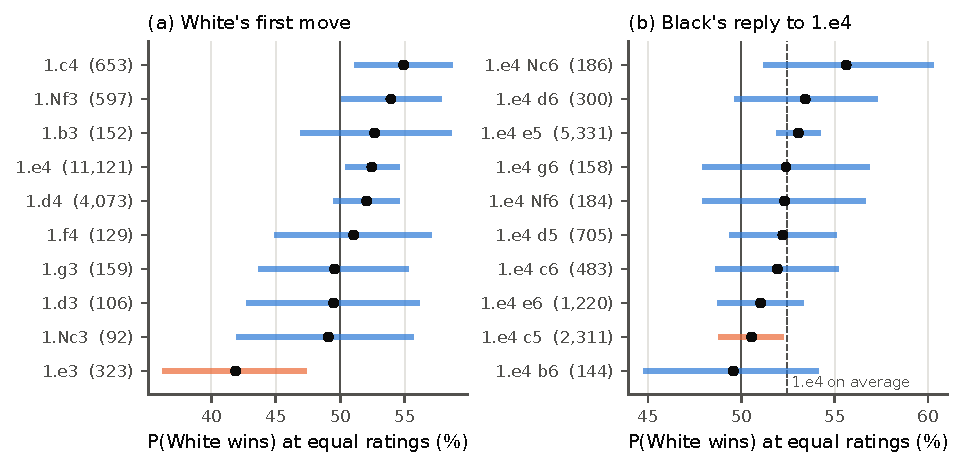
\includegraphics[width=\linewidth]{moves.pdf}
  \caption{White's chance of winning a decisive game against an opponent of the same rating, from the model of White's first move and Black's reply, each chosen by one player alone. Dots are posterior means and bars 90\% intervals, in orange for the two moves discussed below; the number of decisive games is in parentheses. (a): first moves with at least 90 games. 1.e3 is clearly worse for White (41.9\%, 36.2 to 47.4\%), and 1.c4 the best of the common moves (54.9\%). (b): replies to 1.e4 with at least 140 games; the dashed line is 1.e4 on average. After the Sicilian, 1...c5, White wins 50.5\% (48.8 to 52.3\%), against 53.1\% after 1...e5; the posterior probability that the Sicilian is better for Black than 1...e5 is 97.6\%. Overall, White's first move matters more than Black's reply: the spread between first moves, $\sigma_{\text{move}} = 0.22$, exceeds the spread between replies to one first move, $\sigma_{\text{reply}} = 0.13$, with posterior probability 0.90.}
  \label{fig:moves}
\end{figure}
